%%%%%%%%%%%%%%%%%%%%%%%%%%%%%%%%%%%%%%%%%%%%%%%%%%%%%%%%%%%%%
%% Begin exercise %%
%%%%%%%%%%%%%%%%%%%%%%%%%%%%%%%%%%%%%%%%%%%%%%%%%%%%%%%%%%%%%
\ex{Step-down converter and power loss calculation}

%%%%%%%%%%%%%%%%%%%%%%%%%%%%%%%%%%%%%%%%%%%%%%%%%%%%%%%%%%%%%
%% Task 1: Step-down converter without output filter %%
%%%%%%%%%%%%%%%%%%%%%%%%%%%%%%%%%%%%%%%%%%%%%%%%%%%%%%%%%%%%%

\task{Step-down converter without output filter}
An ideal switching transistor is used for loss-free and stepless control of a car's rear window heating.
By varying the duty cycle of the transistor the average value of the heating power can be adjusted. The voltage in the car's electrical system is assumed to be constant with $U_1 = \SI{14}{\volt}$. The heater is dimensioned in such a way
that at its nominal voltage $ U_{\mathrm{2N}} = \SI{14}{\volt}$ it consumes a power of $ P_{\mathrm{LN}} = \SI{500}{\watt}$ and
can be modeled with an ohmic resistor. This circuit is shown in \autoref{fig:step_down_with_load_resistor}.
% figure figCircuitWithOneTransistorAndOneLoadResistor
%%%%%%%%%%%%%%%%%%%%%%%%%%%%%%%%%%%%%%%%%%%%%%%%%%%%%%%%%%%%%%%%%%%%%%%%%%
% CircuitWithOneTransistorAndOneLoadResistor
%%%%%%%%%%%%%%%%%%%%%%%%%%%%%%%%%%%%%%%%%%%%%%%%%%%%%%%%%%%%%%%%%%%%%%%%%%

\begin{figure}[htb]
    \begin{center}
        \begin{circuitikz}[european currents,european resistors,american inductors]
            \draw
            (0,0) coordinate(U+) to [short,-] ++(0.5,0)  
            node[currarrow](Tl){} -- ++(1,0) ++(0.5,0) node[nigfete,rotate=90](Trans){} -- ++(1.5,0) coordinate(Tr)
                to [short,-*] ++(0.5,0) coordinate(junc1)   -- ++(0.5,0) coordinate(Ll) to [L,l_=$L$,i^=$i_\text{L}$]
                ++(2,0) coordinate(Lr) to [short,-*] ++(0.5,0) coordinate(junc2)  -- ++(2,0)
                coordinate(Rt) to [R,l_=$R$,i_=$i_\text{2}$,v^=$U_\text{2}$,voltage shift=0.5, voltage=straight] ++(0,-3) coordinate(Rb)
                to [short,-*] ++(-2,0) coordinate(junc3) to [short,-*] ++(-3,0) coordinate(junc4) to [short] ++(-2,0)
                coordinate(junc5) to [short,-] ++(-2,0) coordinate(U-)
                (junc2) to [C,l_=$C$](junc3)
                (junc4) to [short]  ++(0,0.5) coordinate(Db) to[D-,l^=$D$]  ++(0,2) coordinate(Dt) to [short] (junc1)
                (Trans.G)  to [sqV] ++(0,-1)(junc5) 
            
            (U+) to [V=$U_1$] (U-)
            
            (Trans)  node[anchor=south,color=black]{$T_1$}	
            (Tl)  node[anchor=south,color=black]{$i_\text{1}$}	
            ;
        \end{circuitikz}
    \end{center}
    \caption{Circuit with one transistor, filter and one load resistor.}
    \label{fig:step_down_with_load_resistor}
\end{figure}

\subtask{Draw qualitative current and voltage curves on the load resistor.}
\begin{solutionblock}
The graph \autoref{fig:Currents and voltages during the period} shows the voltages and currents at the load resistor with the period $T_{\mathrm{s}}$, the switch-on time $T_{\mathrm{on}}$ and the switch-off time $T_{\mathrm{off}}$. 

% Solution figure sfigDisplayOfCurrentsAndVoltagesDependingOnTheSwitchingPhases
%%%%%%%%%%%%%%%%%%%%%%%%%%%%%%%%%%%%%%%%%%%%%%%%%%%%%%%%%%%%%%%%%%%%%%%%%%
% DisplayOfCurrentsAndVoltagesDependingOnTheSwitchingPhases
%%%%%%%%%%%%%%%%%%%%%%%%%%%%%%%%%%%%%%%%%%%%%%%%%%%%%%%%%%%%%%%%%%%%%%%%%%

\begin{solutionfigure}[htb]
    \begin{center}
        \begin{tikzpicture}
            \begin{axis}[
                domain=0:15,
                xmin=0, xmax=15,
                ymin=-1, ymax=2.5,
                samples=500,
                axis y line=center,
                axis x line=middle,
                xtick distance=1,
                ytick distance=2,
                extra y ticks=0,
                x label style={at={(axis description cs:1,0.25)},anchor=north},
                y label style={at={(axis description cs:0,.95)},anchor=south},
                width=0.8\textwidth,
                height=0.25\textwidth,
                xlabel={$t$},
                ylabel={{\color{blue}$u_\text{2}(t)$}\quad{\color{red}$i_\text{2}(t)$}},
                xtick={0},
                xticklabels={$0$},
                ytick={0,1,2},
                yticklabels={0,{\color{red}$\frac{U_1}{R_\text{L}}$},{\color{blue}$U_1$}},
                grid=none,
                grid style={line width=.1pt, draw=gray!10},
                major grid style={line width=.2pt,draw=gray!50},    ]
                \addplot[color=red,mark=none,solid] coordinates{
                    (0, 0)
                    (1, 0)
                    (1, 1)
                    (3, 1)
                    (3, 0)
                    (6, 0)
                    (6, 1)
                    (8, 1)
                    (8, 0)
                    (11, 0)
                    (11, 1)
                    (13, 1)
                    (13, 0)
                    (15, 0)
                };
                \addplot[color=blue,mark=none,dashed] coordinates{
                    (0, 0)
                    (1, 0)
                    (1, 2)
                    (3, 2)
                    (3, 0)
                    (6, 0)
                    (6, 2)
                    (8, 2)
                    (8, 0)
                    (11, 0)
                    (11, 2)
                    (13, 2)
                    (13, 0)
                    (15, 0)
                };
            \draw[>=triangle 45, <->] (axis cs:1,0.7) -- (axis cs:3,0.7);
            \node[anchor=north] at (axis cs:2,0.7){$T_\text{on}$};
            \draw[>=triangle 45, <->] (axis cs:3,0.7) -- (axis cs:6,0.7);
            \node[anchor=north] at (axis cs:4.5,0.7){$T_\text{off}$};
            \draw[>=triangle 45, <->] (axis cs:1,-0.3) -- (axis cs:6,-0.3);
            \node[anchor=north] at (axis cs:3.5,-0.3){$T_\text{s}$};
            \end{axis}
        \end{tikzpicture}
    \end{center}
    \caption{Display of currents and voltages depending on the switching phases.}
    \label{fig:Currents and voltages during the period}
\end{solutionfigure}
 


            
\end{solutionblock}

\subtask{Draw the instantaneous power at the load resistor.}


\begin {solutionblock}
The \autoref{fig:Instantaneous power} shows the time curve of the instantaneous power at the load resistor.

% Solution figure sfigInstantaneousPowerAtTheLoadResistor
%%%%%%%%%%%%%%%%%%%%%%%%%%%%%%%%%%%%%%%%%%%%%%%%%%%%%%%%%%%%%%%%%%%%%%%%%%
% InstantaneousPowerAtTheLoadResistor
%%%%%%%%%%%%%%%%%%%%%%%%%%%%%%%%%%%%%%%%%%%%%%%%%%%%%%%%%%%%%%%%%%%%%%%%%%

\begin{solutionfigure}[ht]
    \begin{center}
        \begin{tikzpicture}
        \begin{axis}[
            domain=0:15,
            xmin=0, xmax=15,
            ymin=-1, ymax=2.5,
            samples=500,
            axis y line=center,
            axis x line=middle,
            xtick distance=1,
            ytick distance=2,
            extra y ticks=0,
            x label style={at={(axis description cs:1,0.25)},anchor=north},
            y label style={at={(axis description cs:-.05,.97)},anchor=south},
            width=0.8\textwidth,
            height=0.25\textwidth,
            xlabel={$t$},
            ylabel={{\color{blue}$p(t)$}},
            xtick={0},
            xticklabels={$0$},
            ytick={0,2},
            yticklabels={0,{\color{blue}$\frac{U_1^2}{R_L}$}},
            grid=none,
            grid style={line width=.1pt, draw=gray!10},
            major grid style={line width=.2pt,draw=gray!50},    ]
            \addplot[color=blue,mark=none,solid] coordinates{
                (0, 0)
                (1, 0)
                (1, 2)
                (3, 2)
                (3, 0)
                (6, 0)
                (6, 2)
                (8, 2)
                (8, 0)
                (11, 0)
                (11, 2)
                (13, 2)
                (13, 0)
                (15, 0)
            };
        \draw[>=triangle 45, <->] (axis cs:1,0.7) -- (axis cs:3,0.7);
        \node[anchor=north] at (axis cs:2,0.7){$T_\text{on}$};
        \draw[>=triangle 45, <->] (axis cs:3,0.7) -- (axis cs:6,0.7);
        \node[anchor=north] at (axis cs:4.5,0.7){$T_\text{off}$};
        \draw[>=triangle 45, <->] (axis cs:1,-0.3) -- (axis cs:6,-0.3);
        \node[anchor=north] at (axis cs:3.5,-0.3){$T_\text{s}$};
        \end{axis}
    \end{tikzpicture}
    \end{center}
    \caption{Instantaneous power at the load resistor.}
    \label{fig:Instantaneous power}
\end{solutionfigure}




\end{solutionblock}

\subtask{Derive the relationships for the mean voltage $\overline u_2$, the mean current $\overline i_2$ and the mean power $\overline{p}_{\mathrm{2}}$.}

\begin{solutionblock}
In order to calculate the average voltage $\overline u_2$, the voltage $u_{\mathrm{2}}(t)$ must be integrated over the period $T_{\mathrm{s}}$:

\begin{equation}
    \overline u_2 = \frac{1}{T_{\mathrm{s}}} \int_0^{ T_{\mathrm{s}}} u_2 (t) \, \mathrm{d}t = \frac{1}{ T_{\mathrm{s}}} \int_0^{D T_{\mathrm{s}}} U_1 \, \mathrm{d}t + \frac{1}{ T_{\mathrm{s}}} \int_{D  T_{\mathrm{s}}}^{ T_{\mathrm{s}}} 0 \, \mathrm{d}t$$
    $$= \left . \frac{U_1}{ T_{\mathrm{s}}} t \right |_0^{D  T_{\mathrm{s}}}  + 0 = \frac{U_1 D  T_{\mathrm{s}}}{ T_{\mathrm{s}}} = U_1 D.
\end{equation}

For the mean value $\overline i_2$, the current $i_{\mathrm{2}}(t)$ must be integrated over the period $T_{\mathrm{s}}$:
\begin{equation}
    \overline i_2 = \frac{1}{ T_{\mathrm{s}}} \int_0^{ T_{\mathrm{s}}} i_2(t) \, \mathrm{d}t = \frac{1}{ T_{\mathrm{s}}}\int_0^{D  T_{\mathrm{s}}} \frac{U_1}{ R_{\mathrm{L}}} \, \mathrm{d}t + \frac{1}{ T_{\mathrm{s}}}\int_{D  T_{\mathrm{s}}}^{ T_{\mathrm{s}}} 0 \, \mathrm{d}t$$
    $$= \left . \frac{U_1}{ R_{\mathrm{L}}  T_{\mathrm{on}}}  t \right |_0^{D  T_{\mathrm{s}}} = \frac{U_1 D  T_{\mathrm{s}}}{ R_{\mathrm{L}}  T_{\mathrm{s}}} = \frac{U_1}{ R_{\mathrm{L}}} D.
\end{equation}

To calculate the mean value $\overline{p}_{\mathrm{2}}$, the power $p(t)$ must be integrated over the period $T_{\mathrm{s}}$:
\begin{equation}
    \overline{p}_{\mathrm{2}} = \frac{1}{T_{\mathrm{s}}} \int_0^{T_{\mathrm{s}}} p(t) \mathrm{d}t = \frac{1}{T_{\mathrm{s}}} \int_0^{D T_{\mathrm{s}}} \frac{U_1^2}{ R_{\mathrm{L}}} \mathrm{d}t = \frac{U_1^2 D T_{\mathrm{s}}}{ T_{\mathrm{s}}  R_{\mathrm{L}}} = \frac{U_1^2 D}{ R_{\mathrm{L}}}.
\end{equation}
\end{solutionblock}


\subtask{How large should the duty cycle D be selected so that an average voltage of $\overline u_2 = \SI{8}{\volt}$ is applied to the heater? What is the mean value of the current $\overline i_2$? What power $\overline{p}_{\mathrm{2}}$ is converted into heat?}

\begin {solutionblock}
To determine the duty cycle D, the average voltage $\overline u_2$  must be divided by the source voltage $U_1$
\begin{equation}
    \overline u_2 = D U_1 \quad \Leftrightarrow \quad D = \frac{\overline u_2}{U_1} = \frac{\SI{8}{\volt}}{\SI{14}{\volt}}=0.57.
\end{equation}
    
In order to determine the average current $\overline i_2$, the load resistance $R_{\mathrm{L}}$ must be calculated first:
\begin{equation}
   \overline i_2 = \frac{U_1}{ R_{\mathrm{L}}}  D.
\end{equation}

The known power equation is used to determine the load resistance $R_{\mathrm{L}}$
\begin{equation}
   \quad  P_{\mathrm{LN}} = \frac{{ U_{\mathrm{2N}}}^2}{ R_{\mathrm{L}}} \quad
 \Leftrightarrow \quad R_{\mathrm{L}} = \frac{ U_{\mathrm{2N}}^2}{ P_{\mathrm{LN}}} = \frac{(\SI{14}{\volt})^2}{\SI{500}{\watt}} = \SI{392}{\milli\ohm}.
\end{equation}

Inserting into the current equation delivers :
 $$\overline i_2 = \frac{\SI{14}{\volt}}{\SI{392}{\milli\ohm}} 0.57 =  \SI{20.36}{\ampere}.$$
 
The average power $\overline{p}_{\mathrm{2}}$ yields
 \begin{equation}
 \overline{p}_{\mathrm{2}} = \frac{U_1^2}{ R_{\mathrm{L}}}  D = \frac{(\SI{14}{\volt})^2}{\SI{392}{\milli\ohm}}  0.57 = \SI{285}{\watt}.
\end{equation}
\end{solutionblock}
	
\subtask{When starting the engine, the heater may draw a maximum average current ${\overline i_{2,\mathrm{s}}} = \SI{10}{\ampere}$ from the vehicle electrical system. With which duty cycle $D$ should the transistor be switched in this case?
What is the average voltage $\overline u_2$ at the heater? What power $\overline{p}_{\mathrm{2}}$ is converted into heat?}
\begin{solutionblock}
    Due to the structure of the circuit, it is noticeable that the average current $\overline i_1$ is equal to the average current $\overline i_2$. The corresponding ratio for $\overline i_{2,\mathrm{s}}$ can be calculated from this.
    \begin{equation}
            \overline i_1 = \overline i_2 = \frac{U_1}{R_{\mathrm{L}}}  D \overset ! \leq {\overline i_{\mathrm{2,s}}} \quad \Leftrightarrow \quad  D \leq \frac{{\overline i_{\mathrm{2,s}}}  R_{\mathrm{L}}}{U_1} = \frac{\SI{10}{\ampere} \cdot {\SI{392}{\milli\ohm}}}{\SI{14}{\volt}} = 0.28
    \end{equation}
    
    To determine the average voltage $\overline u_2$ at the heater, the duty cycle D is offset against the source voltage $U_1$.
    \begin{equation}
        \overline u_2 = D  U_1 = 0.28 \cdot \SI{14}{\volt} = \SI{3.92}{\volt}
    \end{equation}
    To determine the power $\overline{p}_{2}$ that is converted into heat, the corresponding duty cycle D must be considered:
     \begin{equation}
        \overline{p}_{\mathrm{2}} = \frac{U_1^2 D}{ R_{\mathrm{L}}} = \frac{(\SI{14}{\volt})^2 \cdot 0.28}{\SI{392}{\milli\ohm}}= \SI{140}{\watt}.   
    \end{equation}
\end{solutionblock}


\subtask{During the journey, the heat output should be $ \overline{p}_{\mathrm{2,f}} = \SI{200}{\watt}$. How is the duty cycle
	 $D$ set? What are the mean values of the current $\overline i_\mathrm{2}$ and the voltage $\overline u_\mathrm{2}$?}
\begin{solutionblock}
To determine the duty cycle D, the familiar power formula is applied:
\begin{equation}
    \overline{p}_{\mathrm{2,f}} \overset ! = \frac{U_\mathrm{1}^2}{ R_{\mathrm{L}}} D \quad 
    \Leftrightarrow \quad D = \frac{ R_{\mathrm{L}}  \overline{p}_{\mathrm{2,f}}}{U_\mathrm{1^2}} = \frac{\SI{392}{\milli\ohm} \cdot \SI{200}{\watt}}{(\SI{14}{\volt})^2} = 0.4.
\end{equation}
The known equations are used to determine the average current $\overline i_\mathrm{2}$ and the average voltage $\overline u_\mathrm{2}$:
\begin{equation}
    \overline i_\mathrm{2} = \frac{U_\mathrm{1}}{ R_{\mathrm{L}}} D = \frac{\SI{14}{\volt}}{\SI{392}{\milli\ohm}} \cdot 0.4 = \SI{14.29}{\ampere},
\end{equation}
\begin{equation}
 \overline u_\mathrm{2} = U_\mathrm{1} D = {\SI{14}{\volt}} \cdot 0.4 = \SI{5.6}{\volt}.
\end{equation}
\end{solutionblock}

%%%%%%%%%%%%%%%%%%%%%%%%%%%%%%%%%%%%%%%%%%%%%%%%%%%%%%%%%%%%%
%% Task 2: Step-down converter with output filter %%
%%%%%%%%%%%%%%%%%%%%%%%%%%%%%%%%%%%%%%%%%%%%%%%%%%%%%%%%%%%%%

\task{Step-down converter with output filter}
A step-down converter is used to charge a mobile phone from the vehicle electrical system with the vehicle electrical system voltage $U_1 = \SI{13.5}{\volt}$. The input voltage of the mobile phone is $U_2 = \SI{4.5}{\volt}$. Consider both voltages as constant, the inductance of the coil is $L = \SI{10}{\micro\henry}$ and the switching frequency is $f_\mathrm{s} = \SI{ 100}{\kilo\hertz}$. All components are considered ideal.

% figure figStepDownConverterOutputFilter
%%%%%%%%%%%%%%%%%%%%%%%%%%%%%%%%%%%%%%%%%%%%%%%%%%%%%%%%%%%%%%%%%%%%%%%%%%
% StepDownConverterOutputFilter
%%%%%%%%%%%%%%%%%%%%%%%%%%%%%%%%%%%%%%%%%%%%%%%%%%%%%%%%%%%%%%%%%%%%%%%%%%

\begin{figure}[htb]
    \begin{center}
        \begin{circuitikz}[european currents,european resistors,american inductors]
            \draw
            (0,0) coordinate(U+) to [short,-] ++(0.5,0)  
            node[currarrow](Tl){} -- ++(1,0) ++(0.5,0) node[nigfete,rotate=90](Trans){} -- ++(1.5,0) coordinate(Tr)
                to [short,-*] ++(0.5,0) coordinate(junc1)   -- ++(0.5,0) coordinate(Ll) to [L,l_=$L$,i^=$i_\text{L}$]
                ++(2,0) coordinate(Lr) to [short,-*] ++(0.5,0) coordinate(junc2)  -- ++(2,0)
                coordinate(Rt) to [R,l_=$R$,i_=$i_\text{2}$,v^=$U_\text{2}$,voltage shift=0.5, voltage=straight] ++(0,-3) coordinate(Rb)
                to [short,-*] ++(-2,0) coordinate(junc3) to [short,-*] ++(-3,0) coordinate(junc4) to [short] ++(-2,0)
                coordinate(junc5) to [short,-] ++(-2,0) coordinate(U-)
                (junc2) to [C,l_=$C$](junc3)
                (junc4) to [short]  ++(0,0.5) coordinate(Db) to[D-,l^=$D$]  ++(0,2) coordinate(Dt) to [short] (junc1)
                (Trans.G)  to [sqV] ++(0,-1)(junc5) 
            
            (U+) to [V=$U_1$] (U-)
            
            (Trans)  node[anchor=south,color=black]{$T_1$}	
            (Tl)  node[anchor=south,color=black]{$i_\text{1}$}	
            ;
        \end{circuitikz}
    \end{center}
    \caption{Circuit with one transistor, filter and one load resistor.}
    \label{fig:step_down_converter_output_filter}
\end{figure}





\subtask{Draw the equivalent circuits for the two switching states.}
% Solution of subtask

\begin{solutionblock}

% solution figure sfigSwitchingStatesStepDownConverter
%%%%%%%%%%%%%%%%%%%%%%%%%%%%%%%%%%%%%%%%%%%%%%%%%%%%%%%%%%%%%%%%%%%%%%%%%%
% SwitchingStatesStepDownConverter
%%%%%%%%%%%%%%%%%%%%%%%%%%%%%%%%%%%%%%%%%%%%%%%%%%%%%%%%%%%%%%%%%%%%%%%%%%

\begin{solutionfigure}[ht]
    \centering
    \begin{tabular}{cc}
            transistor conducts & diode conducts\\
        \begin{circuitikz}[european currents,european resistors,american inductors,]
            \draw
            (0,0) coordinate(u1o)
            to [V,v^=$U_2$] ++(0,-3) coordinate(u1u)
                (u1o) to [short,-,i^<=$i_2$] ++(-1,0) to [L,l_=$L$,v^<=$u_\text{L}$,mirror,voltage=straight] ++(-3,0) to [short,-,i^<=$i_1$] ++(-1,0) coordinate(uqo)
                (u1u) to [short,-] ++(-5,0) coordinate(uqu)
                (uqo) to [V,v_=$U_1$] (uqu)
                ;
        \end{circuitikz}
    &
        \begin{circuitikz}[european currents,european resistors,american inductors,]
            \draw
            (0,0) coordinate(u2o)
            to [V,v^=$U_2$, voltage=straight] ++(0,-3) coordinate(u2u)
                (u2o) to [short,-,i^<=$i_2$] ++(-1,0) to [L,l_=$L$,v^<=$u_\text{L}$,mirror,voltage=straight] ++(-3,0) coordinate(Ll) ++(-1,0) coordinate(uqo)
                (u2u) to [short,-*] ++(-4,0) coordinate(Llu) to [short,-] ++(-1,0) coordinate(uqu)
                (Llu) to [short,-,i_=$i_1$] (Ll)
                (uqo) to [V,v_=$U_1$] (uqu)
                ;
        \end{circuitikz}
    \end{tabular}
    \caption{Circuits for different switching states.}
    \label{fig:switching_states_step-down_converter}
\end{solutionfigure}





\end{solutionblock}

\subtask{At what duty cycle $D$ should the buck converter be operated?}
% Solution of subtask
\begin{solutionblock}
    The duty cycle corresponds to the relation of output voltage to input voltage:
    \begin{equation}
        D = \frac{U_2}{U_1} = \frac{\SI{ 4.5}{\volt}}{\SI{ 13.5}{\volt}} = \frac{1}{3}.
    \end{equation}
\end{solutionblock}
   
\subtask{Sketch the voltage and current signals in the components.}
% Solution of subtask
\begin{solutionblock} %[htb]
The signals of $u_\mathrm{T}$, $u_\mathrm{D}$, $u_\mathrm{L}$, $i_\mathrm{L}$ and $i_\mathrm{T}$ are displayed in \autoref{fig:transistor_circuit}.

% solution figure sfigRelevantVoltageAndCurrentSignals
%%%%%%%%%%%%%%%%%%%%%%%%%%%%%%%%%%%%%%%%%%%%%%%%%%%%%%%%%%%%%%%%%%%%%%%%%%
% RelevantVoltageAndCurrentSignals
%%%%%%%%%%%%%%%%%%%%%%%%%%%%%%%%%%%%%%%%%%%%%%%%%%%%%%%%%%%%%%%%%%%%%%%%%%

\begin{solutionfigure}[htb]  
    \begin{center}
        \definecolor{orange}{rgb}{1.0,0.5,0}
        \begin{tikzpicture}
            % groupplot begin
            \begin{groupplot}[group style={
                        group size=1 by 5,
                        xlabels at=edge bottom,
                        y descriptions at=edge left,
                    },
                    xmin=0, xmax=13.5,
                    domain=0:13,
                    width=0.6\textwidth,
                    xtick={0,1,4,5,8,9,12,13},
                    xticklabels={{},{},{},{},{},{},{},{},{},{}},
                    grid=both,
                    grid style={line width=.1pt, draw=gray!10},
                    major grid style={line width=.2pt,draw=gray!50},    
                    axis y line=center,
                    axis x line=middle,
                ]

                \nextgroupplot[
                    ymin=0, ymax=1.2,
                    samples=500,
                    ytick distance=2,
                    extra y ticks=0,
                    x label style={at={(axis description cs:1,0)},anchor=north},
                    y label style={at={(axis description cs:-.05,.97)},anchor=south},
                    height=0.2\textwidth,
                    xlabel={$t$},
                    ylabel={{\color{orange}$u_\text{T}$}},
                    ytick={0,1},
                    yticklabels={0,$U_1$},
                ]
                \addplot[color=orange,mark=none,solid] coordinates{
                    (0, 0)
                    (1, 0)
                    (1, 1)
                    (4, 1)
                    (4, 0)
                    (5, 0)
                    (5, 1)
                    (8, 1)
                    (8, 0)
                    (9, 0)
                    (9, 1)
                    (12,1)
                    (12,0)
                    (13, 0)
                };  
                    
                \nextgroupplot[
                    ymin=0, ymax=1.2,
                    samples=500,
                    axis y line=center,
                    ytick distance=2,
                    extra y ticks=0,
                    x label style={at={(axis description cs:1,0)},anchor=north},
                    y label style={at={(axis description cs:-.05,.97)},anchor=south},
                    height=0.2\textwidth,
                    xlabel={$t$},
                    ylabel={{\color{blue}$u_\text{D}$}},
                    ytick={0,.33,1},
                    yticklabels={0,$U_2$,$U_1$},
                ]
                \addplot[color=blue,mark=none,solid] coordinates{
                    (0, 1)
                    (1, 1)
                    (1, 0)
                    (4, 0)
                    (4, 1)
                    (5, 1)
                    (5, 0)
                    (8, 0)
                    (8, 1)
                    (9, 1)
                    (9, 0)
                    (12,0)
                    (12,1)
                    (13, 1)
                    (13, 0)
                };
                
                \nextgroupplot[
                    ymin=-.5, ymax=1.2,
                    samples=500,
                    axis y line=center,
                    ytick distance=2,
                    extra y ticks=0,
                    x label style={at={(axis description cs:1,0.25)},anchor=north},
                    y label style={at={(axis description cs:-.05,.97)},anchor=south},
                    height=0.25\textwidth,
                    xlabel={$t$},
                    ylabel={{\color{orange}$u_\text{L}$}},
                    ytick={-.333,0,1},
                    yticklabels={$-U_2$,0,$U_1-U_2$},
                ]
                \draw [fill=green] (axis cs:4,0) rectangle (axis cs:5,1);
                \draw [fill=cyan] (axis cs:5,0) rectangle (axis cs:8,-.3333);
                \addplot[color=orange,mark=none,solid] coordinates{
                    (0, 1)
                    (1, 1)
                    (1, -.333)
                    (4, -.333)
                    (4, 1)
                    (5, 1)
                    (5, -.333)
                    (8, -.333)
                    (8, 1)
                    (9, 1)
                    (9, -.333)
                    (12, -.333)
                    (12, 1)
                    (13, 1)
                    (13, -.333)
                };
                \node[anchor=center] at (axis cs:4.5,0.5){\tiny $ A_\text{off}$};
                \node[anchor=center] at (axis cs:6.5,-0.1667){\tiny $ A_\text{on}$};

                \nextgroupplot[
                    ymin=0, ymax=1.2,
                    samples=500,
                    axis y line=center,
                    ytick distance=2,
                    extra y ticks=0,
                    x label style={at={(axis description cs:1,0)},anchor=north},
                    y label style={at={(axis description cs:-.05,.97)},anchor=south},
                    height=0.2\textwidth,
                    xlabel={$t$},
                    ylabel={{\color{red}$i_\text{L}$}},
                    ytick={0,.5,.75,1},
                    yticklabels={0,,,},
                ]
                \addplot[color=red,mark=none,solid] coordinates{
                    (0, 0.5)
                    (1, 1)
                    (4, 0.5)
                    (5, 1)
                    (8, 0.5)
                    (9, 1)
                    (12,0.5)
                    (13,1)
                };

                \nextgroupplot[
                    ymin=0, ymax=1.2,
                    samples=500,
                    axis y line=center,
                    ytick distance=2,
                    extra y ticks=0,
                    x label style={at={(axis description cs:1,0)},anchor=north},
                    y label style={at={(axis description cs:-.0,.97)},anchor=south},
                    height=0.2\textwidth,
                    xlabel={$t$},
                    ylabel={{\color{orange}$i_\text{T}$}\quad{\color{blue}$i_\text{D}$}},
                    ytick={0,.5,.75,1},
                    yticklabels={0,,,},
                ]
                \addplot[color=orange,mark=none,solid] coordinates{
                    (0,0)
                    (0, 0.5)
                    (1, 1)
                    (1, 0)
                    (4,0)
                    (4,0.5)
                    (5, 1)
                    (5,0)
                    (8,0)
                    (8, 0.5)
                    (9, 1)
                    (9,0)
                    (12,0)
                    (12,0.5)
                    (13,1)
                    (13,0)
                };
                \addplot[color=blue,mark=none,solid] coordinates{
                    (1,1)
                    (4, 0.5)
                };
                \addplot[color=blue,mark=none,solid] coordinates{
                    (5,1)
                    (8, 0.5)
                };
                \addplot[color=blue,mark=none,solid] coordinates{
                    (9,1)
                    (12, 0.5)
                };
                \addplot[color=blue,mark=none,solid] coordinates{
                    (0,0)
                    (1, 0)
                };
                \addplot[color=blue,mark=none,solid] coordinates{
                    (4,0)
                    (5,0)
                };
                \addplot[color=blue,mark=none,solid] coordinates{
                    (8,0)
                    (9,0)
                };
                \addplot[color=blue,mark=none,solid] coordinates{
                    (12,0)
                    (13,0)
                };
                \addplot[color=blue,mark=none,dashed] coordinates{
                    (1,0)
                    (1,1)
                };
                \addplot[color=blue,mark=none,dashed] coordinates{
                    (4,0)
                    (4,0.5)
                };
                \addplot[color=blue,mark=none,dashed] coordinates{
                    (5,0)
                    (5,1)
                };
                \addplot[color=blue,mark=none,dashed] coordinates{
                    (8,0)
                    (8,0.5)
                };
                \addplot[color=blue,mark=none,dashed] coordinates{
                    (9,0)
                    (9,1)
                };
                \addplot[color=blue,mark=none,dashed] coordinates{
                    (12,0)
                    (12,0.5)
                };
                \addplot[color=blue,mark=none,dashed] coordinates{
                    (13,0)
                    (13,1)
                };
            \end{groupplot}
        \end{tikzpicture}
    \end{center}
    \caption{Relevant voltage and current signals.}
    \label{fig:transistor_circuit}
\end{solutionfigure}       




\end{solutionblock}

\subtask{How large is the current ripple $\Delta i_\mathrm{L}$ of the coil current in boundary conduction mode (BCM) operation?}
% Solution of subtask
\begin{solutionblock}
The BCM operation is characterized by zero inductor current events at the beginning / end of a switching period, compare \autoref{fig:BCM_step-down-converter}.

    % solution figure sfigQualitativeInductorCurrentDuringBCM
    %%%%%%%%%%%%%%%%%%%%%%%%%%%%%%%%%%%%%%%%%%%%%%%%%%%%%%%%%%%%%%%%%%%%%%%%%%
% QualitativeInductorCurrentDuringBCM
%%%%%%%%%%%%%%%%%%%%%%%%%%%%%%%%%%%%%%%%%%%%%%%%%%%%%%%%%%%%%%%%%%%%%%%%%%

\begin{solutionfigure}
    \centering
    \begin{tikzpicture}
        \begin{axis}[
                domain=0:15,
                xmin=0, xmax=7,
                ymin=-1.5, ymax=2.5,
                samples=500,
                axis y line=center,
                axis x line=middle,
                xtick distance=1,
                ytick distance=2,
                extra y ticks=0,
                x label style={at={(axis description cs:1,0.33)},anchor=north},
                y label style={at={(axis description cs:-.05,.97)},anchor=south},
                width=0.6\textwidth,
                height=0.3\textwidth,
                xlabel={$t$},
                ylabel={$i_\text{L}$},
                xtick={0,2,5},
                xticklabels={$0$,{},{}},
                ytick={0,1,2},
                yticklabels={0,$\frac{\Delta i_\text{L}}{2}$,$\Delta i_\text{L}$},
                grid=both,
                grid style={line width=.1pt, draw=gray!10},
                major grid style={line width=.2pt,draw=gray!50},
            ]
            \addplot[color=blue,mark=none,solid] coordinates{
                (0, 0)
                (2, 2)
                (5, 0)
                (7, 2)
            };
            \draw[>=triangle 45, <->] (axis cs:0,-.3) -- (axis cs:2,-.3);
            \node[anchor=north] at (axis cs:1,-.3){$D T_\text{s}$};
            \draw[>=triangle 45, <->] (axis cs:2,-.3) -- (axis cs:5,-.3);
            \node[anchor=north] at (axis cs:3.5,-.3){$(1-D) T_\text{s}$};
            \draw[>=triangle 45, <->] (axis cs:0,-1) -- (axis cs:5,-1);
            \node[anchor=north] at (axis cs:2.5,-1){$T_\text{s}$};
        \end{axis}
    \end{tikzpicture}
    \caption{Qualitative inductor current during BCM}
\end{solutionfigure}






    The relevant switching time intervals are:
    \begin{equation}
        f_\mathrm{s} = \SI{ 100}{\kilo\hertz} \quad \Rightarrow \quad T_\mathrm{s} = \SI{ 10}{\micro\second} \quad \Rightarrow \quad T_\mathrm{on} = D \cdot T_\mathrm{s} = \frac{\SI{ 10}{\micro \second}}{3}.
    \end{equation}
    The (linear) inductor ordinary differential equations yields
    \begin{equation}
        U_\mathrm{L} = U_\mathrm{1} - U_\mathrm{2} = L \frac{\mathrm{d} i_\mathrm{L}}{\mathrm{d}t}  = L \frac{\Delta i_\mathrm{L}}{\Delta t} = L \frac{\Delta i_\mathrm{L}}{T_\mathrm{on}}
    \end{equation}
    resulting to
    \begin{equation}
        \Delta i_\mathrm{L} = \frac{U_\mathrm{1} - U_\mathrm{2}}{L} T_\mathrm{on} = \frac{\SI{13.5}{\volt} - \SI{4.5}{\volt}}{\SI{10}{\micro \henry} \cdot \frac{\SI{10}{\micro \second}}{3}} = \SI{3}{\ampere}
    \end{equation}
    and finally
    \begin{equation}
        I_{\mathrm{2,min}} = \frac{\Delta i_\mathrm{L}}{2} = \SI{1.5}{\ampere}.
    \end{equation}
\end{solutionblock}

\subtask{How large is the worst-case current ripple?}
% Solution of subtask
\begin{solutionblock}
    The worst case ripple is at $D=0.5$ leading to
    \begin{equation}
        U_\mathrm{2} = D U_\mathrm{1},
    \end{equation}
    \begin{equation}
        \Delta i_\mathrm{L,max} = \frac{U_\mathrm{1} - U_\mathrm{2}}{L} 0.5 \cdot T_\mathrm{s}
        \Rightarrow \Delta i_\mathrm{L,max} = \frac{\SI{13.5}{\volt} - \SI{6.75}{\volt}}{\SI{13.5}{\micro \henry}} 0.5 \cdot \SI{10}{\micro \second},
    \end{equation}
    \begin{equation}
        \Delta i_{\mathrm{L,min}} = \SI{3.38}{\ampere}.
    \end{equation}
\end{solutionblock}

\subtask{When starting the engine, the input voltage drops to $U_{1,\mathrm{min}} = \SI{ 10}{\volt}$.
The voltage regulator of the buck converter changes the duty cycle so that the output voltage $U_2 = \SI{4.5}{\volt}$ is kept stable.
What duty cycle D is set?}
% Solution of subtask
\begin{solutionblock}
    The new duty cycle results in:
    \begin{equation}    
        D= \frac{U_\mathrm{2}}{U_{\mathrm{1,min}}} = \frac{\SI{4.5}{\volt}}{\SI{10}{\volt}} = 0.45.
    \end{equation}    
\end{solutionblock}

\subtask{Calculate the average and ripple current in BCM mode considering $U_{1,\mathrm{min}}$ at the input.}
% Solution of subtask
\begin{solutionblock}
    The boundary of discontinuous conduction mode depends on the inductance, duty cycle, switching frequency and voltages:
    \begin{equation}
        \Delta i_\mathrm{L} = \frac{U_{\mathrm{1,min}} - U_\mathrm{2}}{L} D T_\mathrm{s} = \frac{(\SI{10}{\volt} - \SI{4.5}{\volt}) \cdot 0.45 \cdot \SI{10}{\micro \second}}{\SI{10}{\micro \henry}} = \SI{2.48}{\ampere},
    \end{equation}
    \begin{equation}
        I_{\mathrm{L,min}} = \frac{\Delta i_\mathrm{L}}{2} = \SI{1.24}{\ampere}.
    \end{equation}
\end{solutionblock}





%%%%%%%%%%%%%%%%%%%%%%%%%%%%%%%%%%%%%%%%%%%%%%%%%%%%%%%%%%%%%
%% Task 3: Power losses within the step-down converter %%
%%%%%%%%%%%%%%%%%%%%%%%%%%%%%%%%%%%%%%%%%%%%%%%%%%%%%%%%%%%%%


\task{Power losses within the step-down converter}
The power loss of a buck converter is to be analyzed. The inductance is so large
that the current ripple in the output current can be neglected, i.e., $ i_{\mathrm{2}}(t) = I_{\mathrm{2}} =\mathrm{const}$. Furthermore, the component values are given in \autoref{table:Parameters of the circuit} and the currents and voltages of the switch-on and switch-off processes in \autoref{fig:Switch-on behavior and switch-off behavior of} and \autoref{fig:Switch-on behavior and switch-off behavior of voltage}. 

% figure figBuckConverterWithOneTransistorAndOneDiode
%%%%%%%%%%%%%%%%%%%%%%%%%%%%%%%%%%%%%%%%%%%%%%%%%%%%%%%%%%%%%%%%%%%%%%%%%%
% BuckConverterWithOneTransistorAndOneDiode
%%%%%%%%%%%%%%%%%%%%%%%%%%%%%%%%%%%%%%%%%%%%%%%%%%%%%%%%%%%%%%%%%%%%%%%%%%

\begin{figure}[ht]
    \begin{center}
        \begin{circuitikz}[european currents,european resistors,american inductors]
            \draw
        (0,0) coordinate(N1) to [short] ++(1.5,0) coordinate(Ud)
        ++(0,-1) node[nigfete](Trans){}
        (Ud) to [short,i=$i_{\mathrm{c}}(t)$] (Trans.drain)
        (Trans.source) to [short,-] ++(0,0) coordinate(U2p)
        node[circ]{}
        to [short,-] ++(0,0) to [L,l^=$L$] ++(3,0) coordinate(Lp) to [short,-] ++(0,-2) coordinate(Lp10)
        (Lp) to [V, v_=$U_2$] (Lp10)
        (Lp) to [open] (Lp10)
        coordinate(Lp10) to  [short,-] ++(-3,0) coordinate(D)
        to [D,l^=$D$, i=$i_{\mathrm{D}}(t)$] ++(0,2)
        (0,-3.77) coordinate(Bw) to [short] ++(3,0) coordinate(U1)
        %(N1) to [V] (Bw)
        (N1) to [V,v_=$U_1$] (Bw)
        ;
        \end{circuitikz}
    \end{center}
    \caption{Buck converter with one transistor and one diode.}
\end{figure}



%
\begin{table}[ht]
    \centering  % Zentriert die Tabelle
    \begin{tabular}{llll}
        \toprule
        \multicolumn{2}{l}{\textbf{General parameters:}} & \multicolumn{2}{l}{\textbf{Diode:}} \\ 
        Input voltage: &  $U_{\mathrm{1}} = \SI{600}{\volt}$ & Forward voltage: & $u_{\mathrm{F}} = \SI{2.7}{\volt}$ \\
        Output current: & $I_2 = \SI{30}{A}$  & Switch-on losses: & $E_{\text{on},\mathrm{D}} = \SI{52}{\micro\joule}$ \\
        Switching frequency: & $f_{\mathrm{s}} = \SI{25}{\kilo\hertz}$  & Switch-off losses: & $E_{\text{off},\mathrm{D}} = \SI{240}{\micro\joule}$ \\
        \midrule
        \multicolumn{2}{l}{\textbf{IGBT:}} & \multicolumn{2}{l}{\textbf{Inductance:}} \\ 
        Collector-emitter voltage: & $u_{\mathrm{on},\mathrm{CE}} = \SI{2.5}{\volt}$ & Copper resistance: & $R_{\text{Cu}} = \SI{45}{\milli\ohm}$  \\
        & &  Iron losses: & $P_{\mathrm{l},\text{Fe}} = \SI{13}{\watt}$ \\
        \bottomrule
    \end{tabular}
    \caption{Parameters of the circuit.}  % Beschriftung der Tabelle
    \label{table:Parameters of the circuit}
\end{table}
%

% figure figSwitchOnBehaviorAndSwitchOffBehaviorOfUI
%%%%%%%%%%%%%%%%%%%%%%%%%%%%%%%%%%%%%%%%%%%%%%%%%%%%%%%%%%%%%%%%%%%%%%%%%%
% SwitchOnBehaviorAndSwitchOffBehaviorOfUI
%%%%%%%%%%%%%%%%%%%%%%%%%%%%%%%%%%%%%%%%%%%%%%%%%%%%%%%%%%%%%%%%%%%%%%%%%%

    \begin{figure}[ht]
        \centering
        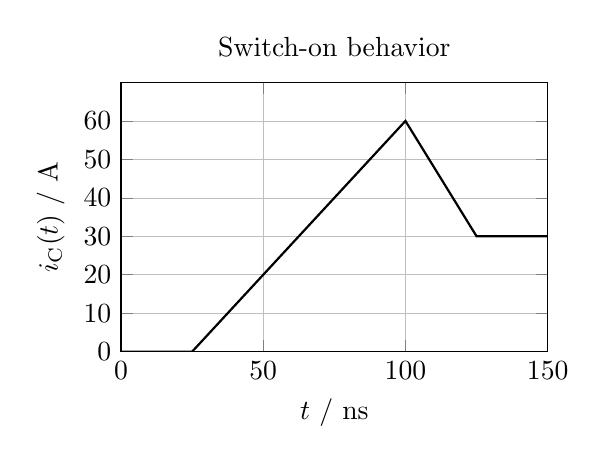
\begin{tikzpicture}
        \begin{axis}[
            width=7cm, height=5cm,
            grid=both,
            major grid style={line width=.2pt,draw=gray!50},
            minor grid style={line width=.1pt,draw=gray!20},
            xlabel={$t$ / ns},
            ylabel={$i_\mathrm{C}(t)$ / A},
            title={Switch-on behavior},
            xmin=0, xmax=150,
            ymin=0, ymax=70,
            xtick={0, 50, 100, 150},
            ytick={0, 10, 20, 30, 40, 50, 60},
            ]
            % Einschaltverhalten graph
            \addplot[
                thick,
                mark=none,
                color=black,
            ] coordinates {
                (0,0) (25,0) (50, 20) (75, 40) (100, 60) (125, 30) (150, 30)
            };
        \end{axis}
        \end{tikzpicture} 
        \hspace{1cm} % Abstand zwischen den beiden Diagrammen
        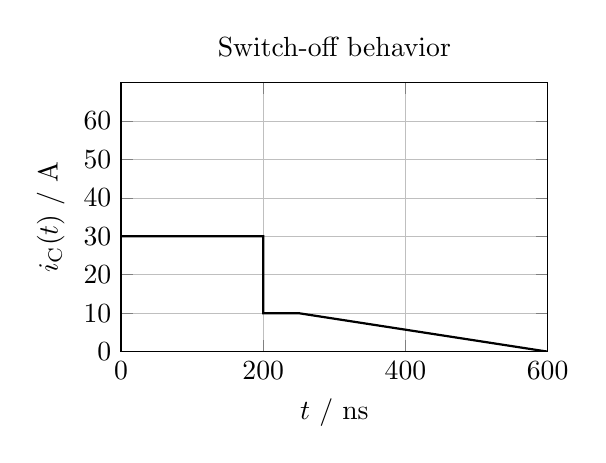
\begin{tikzpicture}
        \begin{axis}[
            width=7cm, height=5cm,
            grid=both,
            major grid style={line width=.2pt,draw=gray!50},
            minor grid style={line width=.1pt,draw=gray!20},
            xlabel={$t$ / ns},
            ylabel={$i_\mathrm{C}(t)$ / A},
            title={Switch-off behavior},
            xmin=0, xmax=600,
            ymin=0, ymax=70,
            xtick={0, 200, 400, 600},
            ytick={0, 10, 20, 30, 40, 50, 60},
            ]
            % Ausschaltverhalten graph
            \addplot[
                thick,
                mark=none,
                color=black,
            ] coordinates {
                (0,30) (200, 30) (200, 10) (250, 10) (600, 0)
            };
        \end{axis}
        \end{tikzpicture}
        \caption{Switch-on behavior and switch-off behavior of $i_{\mathrm{C}}(t)$}
        \label{fig:Switch-on behavior and switch-off behavior of}
    
        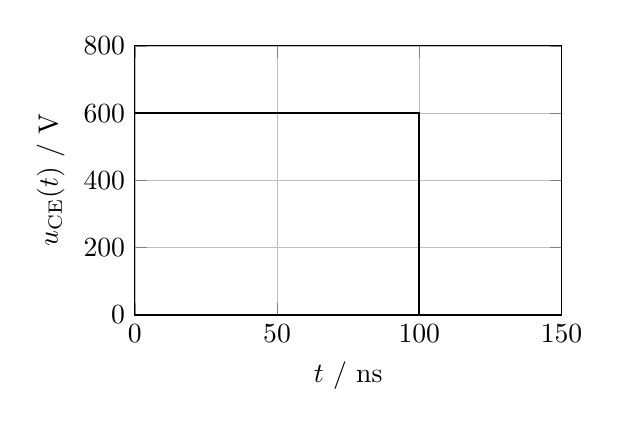
\begin{tikzpicture}
        \begin{axis}[
            width=7cm, height=5cm,
            grid=both,
            major grid style={line width=.2pt,draw=gray!50},
            minor grid style={line width=.1pt,draw=gray!20},
            xlabel={$t$ / ns},
            ylabel={$u_{\mathrm{CE}}(t)$ / V},
            xmin=0, xmax=150,
            ymin=0, ymax=800,
            xtick={0, 50, 100, 150},
            ytick={0,200, 400, 600, 800},
            ]
            % Einschaltverhalten graph
            \addplot[
                thick,
                mark=none,
                color=black,
            ] coordinates {
                (0,600) (100, 600) (100, 0)
            };
        \end{axis}
        \end{tikzpicture}
        \hspace{1cm} % Abstand zwischen den beiden Diagrammen
        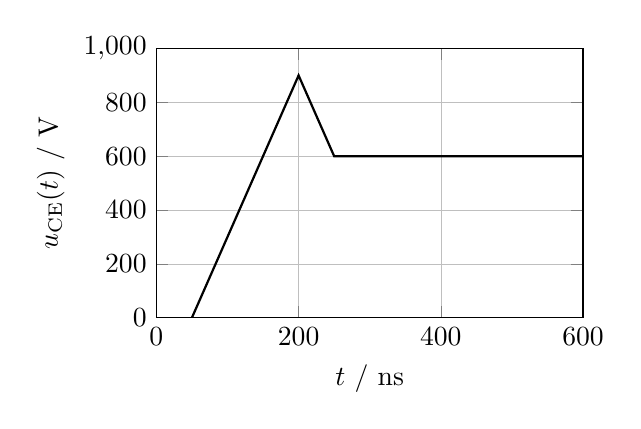
\begin{tikzpicture}
        \begin{axis}[
            width=7cm, height=5cm,
            grid=both,
            major grid style={line width=.2pt,draw=gray!50},
            minor grid style={line width=.1pt,draw=gray!20},
            xlabel={$t$ / ns},
            ylabel={$u_{\mathrm{CE}}(t)$ / V},
            xmin=0, xmax=600,
            ymin=0, ymax=1000,
            xtick={0,200, 400, 600},
            ytick={0,200, 400, 600,800, 1000},
            ]
            % Ausschaltverhalten graph
            \addplot[
                thick,
                mark=none,
                color=black,
            ] coordinates {
                (50,0) (200, 900) (250, 600) (600, 600)
            };
        \end{axis}
        \end{tikzpicture}
        \caption{Switch-on behavior and switch-off behavior of $u_{\mathrm{CE}}(t)$.}
        \label{fig:Switch-on behavior and switch-off behavior of voltage}
    \end{figure}


\subtask{Calculate the switch-on and switch-off loss work $E_{\mathrm{on,T}}$ and $E_{\mathrm{off,T}}$  of the IGBT.}
\begin{solutionblock}
First, the power values for the switch-on process at the times $t = \SI{25}{\ns}$ and $ t = \SI{100}{\ns}$ are calculated:

\begin{equation}
    p(t = \SI{25}{\ns}) = \SI{600}{\volt} \cdot \SI{0}{\ampere} = 0,
\end{equation}

\begin{equation}
    p(t = \SI{100}{\ns}) = \SI{600}{\volt} \cdot \SI{60}{\ampere} = \SI{36}{\kilo\watt}. 
\end{equation}
\autoref{fig:Power values for the switch-on process}  results from these power values.
The switch-on losses of the IGBT can be calculated based on the triangular signal shapes of the provided signals:
        
\begin{equation}
E_{\mathrm{on,T}} = \frac{1}{2} \Delta P \Delta t = \frac{1}{2} \SI{36}{\kilo\watt} \cdot \SI{75}{\ns} = \SI {1.35}{\milli\joule}.
\end{equation}

The switch-off power can now be determined for the times $t = \SI{200}{\ns}$, $t = \SI{200.1}{\ns}$ and $t = \SI{250}{\ns}$:

\begin{equation}
    p(t = \SI{200}{\ns}) = \SI{900}{\volt} \cdot \SI{30}{\ampere} = \SI{27}{\kilo\watt}, 
\end{equation}

\begin{equation}
    p(t = \SI{200.1}{\ns}) = \SI{900}{\volt} \cdot \SI{10}{\ampere} = \SI{9}{\kilo\watt}, 
\end{equation}

\begin{equation}
    p(t = \SI{250}{\ns}) = \SI{600}{\volt} \cdot \SI{10}{\ampere} = \SI{6}{\kilo\watt}. 
\end{equation}

Finally, \autoref{fig:Power values for the switch-off process} results from these power values. The switch-off losses of the IGBT are calculated next. For this purpose, the power curve is divided into three parts:
        
\begin{equation}
E_{\mathrm{off,T}} = E_{\mathrm{1}} + E_{\mathrm{2}} + E_{\mathrm{3}}
\end{equation}
with
\begin{equation}
E_{\mathrm{1}} = \frac{1}{2} \SI{27}{\kilo\watt} \cdot \SI{150}{\ns} = \SI {2.025}{\milli\joule},
\end{equation}
\begin{equation}
E_{\mathrm{2}} = \SI{6}{\kilo\watt} \cdot \SI{50}{\ns} + \frac{1}{2} \SI{3}{\kilo\watt} \cdot \SI{50}{\ns} = \SI {0.375}{\milli\joule},
\end{equation}
\begin{equation}
    E_{\mathrm{3}} = \frac{1}{2} \SI{6}{\kilo\watt} \cdot \SI{350}{\ns} = \SI {1.05}{\milli\joule}.
    \end{equation}
If all three loss work terms are added together, the result is the total switch-off loss work:
\begin{equation}
    E_{\mathrm{off,T}} =  \SI {3.45}{\milli\joule}.
\end{equation}

    % solution figure sfigSwitchOnBehaviorAndSwitchOffBehaviorOfPower
    %%%%%%%%%%%%%%%%%%%%%%%%%%%%%%%%%%%%%%%%%%%%%%%%%%%%%%%%%%%%%%%%%%%%%%%%%%
% SwitchOnBehaviorAndSwitchOffBehaviorOfPower
%%%%%%%%%%%%%%%%%%%%%%%%%%%%%%%%%%%%%%%%%%%%%%%%%%%%%%%%%%%%%%%%%%%%%%%%%%

\begin{solutionfigure}[ht]
    \centering
    \begin{subfigure}[t]{0.45\textwidth}
        \centering
        \begin{tikzpicture}
            \begin{axis}[
                width=7cm, height=5cm,
                grid=both,
                major grid style={line width=.2pt,draw=gray!50},
                minor grid style={line width=.1pt,draw=gray!20},
                xlabel={$t$ / ns},
                ylabel={$p(t)$ / kW},
                xmin=0, xmax=150,
                ymin=0, ymax=45,
                xtick={0, 50, 100, 150},
                ytick={0,9, 18, 27, 36, 45},
            ]
            % Einschaltverhalten graph
            \addplot[
                thick,
                mark=none,
                color=signalalpha,
            ] coordinates {
                (25,0) (100, 36) (100, 0)
            };
            \end{axis}
        \end{tikzpicture}
        \caption{Power values for the switch-on process.}
        \label{fig:Power values for the switch-on process}
    \end{subfigure}
    \hfill % Abstand zwischen den Subfiguren
    \begin{subfigure}[t]{0.45\textwidth}
        \centering
        \begin{tikzpicture}
            \begin{axis}[
                width=7cm, height=5cm,
                grid=both,
                major grid style={line width=.2pt,draw=gray!50},
                minor grid style={line width=.1pt,draw=gray!20},
                xlabel={$t$ / ns},
                ylabel={$p(t)$ / kW},
                xmin=0, xmax=600,
                ymin=0, ymax=45,
                xtick={0,200, 400, 600},
                ytick={0,9, 18, 27,36, 45},
            ]
            % Ausschaltverhalten graph
            \addplot[
                thick,
                mark=none,
                color=signalalpha,
            ] coordinates {
                (50,0) (200, 27) (200, 9) (250, 7) (600,0)
            };
            \end{axis}
        \end{tikzpicture}
        \caption{Power values for the switch-off process.}
        \label{fig:Power values for the switch-off process}
    \end{subfigure}
    \caption{Switch-on behavior and switch-off behavior of $p(t)$.}
\end{solutionfigure}



\end{solutionblock}


\subtask{Calculate the (average) switching power loss in the IGBT $P_{\mathrm{l,sw,T}}$ and in the diode $P_{\mathrm{l,sw,D}}$.}
\begin{solutionblock}
The switching power loss of the IGBT is dependent on the switching frequency $f_{\mathrm{s}}$ in addition to the switch-on and switch-off power losses:
\begin{equation}
    P_{\mathrm{l,sw,T}} =  (E_{\mathrm{on,T}} +  E_{\mathrm{off,T}}) \cdot f_{\mathrm{s}} = (\SI {1.35}{\milli\joule} + \SI {3.45}{\milli\joule}) \cdot \SI {25}{\kilo\hertz} = \SI {120}{\watt}.
 \end{equation}

 Likewise, the switching power loss of the diode also depends on the switching frequency $f_{\mathrm{s}}$:
 \begin{equation}
    P_{\mathrm{l,sw,D}} =  (E_{\mathrm{on,D}} +  E_{\mathrm{off,D}}) \cdot f_{\mathrm{s}} = (\SI {52}{\micro\joule} + \SI {3.45}{\micro\joule}) \cdot \SI {25}{\kilo\hertz} = \SI {7.3}{\watt}.
 \end{equation}
\end{solutionblock}

\subtask{Calculate the (average) conduction losses in the IGBT  $P_{\mathrm{l,cond,T}}(D)$ and in the diode $P_{\mathrm{l,cond,D}}(D)$.}
\begin{solutionblock}
There are two operating states, one in which the IGBT is closed and another in which it is open. Therefore, the IGBT and diode never carry a current at the same time. This means that the conduction losses of the IGBT only occur when it is switched on:
\begin{equation}
    P_{\mathrm{l,cond,T}}(D) = u_{\mathrm{CE,on}} I_\mathrm{2}  D = \SI {2.5}{\volt}\cdot \SI {30}{\ampere} \cdot D = \SI {75}{\watt} \cdot D .
\end{equation}
Furthermore, this means that the forward losses of the diode only occur when the IGBT is switched off:
\begin{equation}
    P_{\mathrm{l,cond,D}}(D)= u_{\mathrm{f}} I_\mathrm{2} (1-D)= \SI {2.7}{\volt}\cdot \SI {30}{\ampere} \cdot (1-D) = \SI {81}{\watt} \cdot (1-D) .
    \end{equation}
\end{solutionblock}

\subtask{Calculate the efficiency $\eta(U_2)$ as a function of the output voltage.}
\begin{solutionblock}
To determine the efficiency, the general equation $\eta=\frac{P_{\mathrm{out}}}{P_{\mathrm{in}}}$ is used
\begin{equation}
    \eta=\frac{P_{\mathrm{out}}}{P_{\mathrm{in}}} = \frac{U_\mathrm{2} I_\mathrm{2}}{U_\mathrm{2} I_\mathrm{2} + P_{\mathrm{l,total}}(D)}
\end{equation}
where $P_{\mathrm{l,total}}(D)$ results from all losses:
\begin{equation}
    P_{\mathrm{l,total}}(D) =  P_{\mathrm{l,sw,T}} +  P_{\mathrm{l,sw,D}} + P_{\mathrm{l,cond,T}}(D) + P_{\mathrm{l,cond,D}}(D) + P_{\mathrm{l,L}}.
\end{equation}
The losses inside the inductor are:
\begin{equation}
   P_{\mathrm{l,L}} = R_{\mathrm{Cu}} (I_{\mathrm{2}})^2 + P_{\mathrm{l,Fe}} = \SI{45}{\mohm} \cdot {(30\ \si{A})^2} + \SI {13}{\watt} = \SI {53.5}{\watt},
\end{equation}
where $P_{\mathrm{l,cond,T}}(D)$ and $P_{\mathrm{l,cond,D}}(D)$ can only be determined in general terms:
\begin{equation}
    P_{\mathrm{l,cond,T}}(D) + P_{\mathrm{l,cond,D}}(D) = I_2( u_{\mathrm{CE,on}} D + u_{\mathrm{F}}(1-D)) = D I_\mathrm{2}(u_{\mathrm{CE,on}} - u_{\mathrm{F}} ) + I_\mathrm{2} u_{\mathrm{F}}.
\end{equation}
Summarizing all power loss components yields:
\begin{equation}
    P_{\mathrm{l,total}}(D) = P_{\mathrm{l,sw,T}}  +  P_{\mathrm{l,sw,D}}  + P_{\mathrm{l,L}} + D I_\mathrm{2}(u_{\mathrm{CE,on}} - u_{\mathrm{F}} ) + I_\mathrm{2} u_{\mathrm{F}} =  P_{\mathrm{l,const}} + D I_\mathrm{2} (u_{\mathrm{CE,on}} - u_{\mathrm{F}})
\end{equation}
The value $P_{\mathrm{l,const}}$ is considering all losses that could be calculated:
\begin{equation}
    P_{\mathrm{l,const}} = \SI {120}{\watt} + \SI {7.3}{\watt} +\SI {53.5}{\watt} + \SI {2.7}{\volt}\cdot\SI {30}{\ampere}.
\end{equation}
\end{solutionblock}

\subtask{The circuit is to be evaluated at   $ U_{\mathrm{2}} = \SI{300}{\volt}$. Calculate the total power loss in the IGBT $P_{\mathrm{l,T}}$ and in the diode $P_{\mathrm{l,D}}$.}
\begin{solutionblock}
Firstly, the duty cycle must be determined:
\begin{equation}
    D = \frac{U_\mathrm{2}}{U_\mathrm{1}} = \frac{\SI{300}{\volt}}{\SI{600}{\volt}} = 0.5.
\end{equation}
The total power loss of the IGBT is made up of the switching losses and the losses during operation:
\begin{equation}
    P_{\mathrm{l,T}}(D) = u_{\mathrm{CE,on}} I_\mathrm{2} D +  P_{\mathrm{l,sw,T}} = \SI{2.5}{\volt} \cdot \SI{30}{\ampere} \cdot 0.5 + \SI{120}{\watt} = \SI{157.5}{\watt}.
\end{equation}
The total power loss of the diode is made up of the switching losses and the losses during operation:
\begin{equation}
    P_{\mathrm{l,D}}(D) = u_{\mathrm{F}} I_\mathrm{2} (1-D) +  P_{\mathrm{l,sw,D}} = \SI{2.7}{\volt} \cdot \SI{30}{\ampere} \cdot 0.5 + \SI{7.3}{\watt} = \SI{47.8}{\watt}.
\end{equation}
\end{solutionblock}
    